%%% LaTeX Template: Designer's CV
%%%
%%% Source: http://www.howtotex.com/
%%% Feel free to distribute this template, but please keep the referal to HowToTeX.com.
%%% Date: March 2012


%%%%%%%%%%%%%%%%%%%%%%%%%%%%%%%%%%%%%
% Document properties and packages
%%%%%%%%%%%%%%%%%%%%%%%%%%%%%%%%%%%%%
\documentclass[a4paper,12pt,final]{memoir}

% misc
\renewcommand{\familydefault}{bch}	% font
\pagestyle{empty}					% no pagenumbering
\setlength{\parindent}{0pt}			% no paragraph indentation


% required packages (add your own)
\usepackage{flowfram}										% column layout
\usepackage[top=1cm,left=1cm,right=1cm,bottom=1cm]{geometry}% margins
\usepackage{graphicx}										% figures
\usepackage{url}											% URLs
\usepackage[usenames,dvipsnames]{xcolor}					% color
\usepackage{multicol}										% columns env.
	\setlength{\multicolsep}{0pt}
\usepackage{paralist}										% compact lists
\usepackage{tikz}
\usepackage{hyperref}
\hypersetup{colorlinks,urlcolor=blue}
%%%%%%%%%%%%%%%%%%%%%%%%%%%%%%%%%%%%%
% Create column layout
%%%%%%%%%%%%%%%%%%%%%%%%%%%%%%%%%%%%%
% define length commands
\setlength{\vcolumnsep}{\baselineskip}
\setlength{\columnsep}{\vcolumnsep}

% frame setup (flowfram package)
% left frame
\newflowframe{0.2\textwidth}{\textheight}{0pt}{0pt}[left]
	\newlength{\LeftMainSep}
	\setlength{\LeftMainSep}{0.2\textwidth}
	\addtolength{\LeftMainSep}{1\columnsep}
 
% small static frame for the vertical line
\newstaticframe{1.5pt}{\textheight}{\LeftMainSep}{0pt}
 
% content of the static frame
\begin{staticcontents}{1}
\hfill
\tikz{%
	\draw[loosely dotted,color=RoyalBlue,line width=1.5pt,yshift=0]
	(0,0) -- (0,\textheight);}%
\hfill\mbox{}
\end{staticcontents}
 
% right frame
\addtolength{\LeftMainSep}{1.5pt}
\addtolength{\LeftMainSep}{1\columnsep}
\newflowframe{0.7\textwidth}{\textheight}{\LeftMainSep}{0pt}[main01]


%%%%%%%%%%%%%%%%%%%%%%%%%%%%%%%%%%%%%
% define macros (for convience)
%%%%%%%%%%%%%%%%%%%%%%%%%%%%%%%%%%%%%
\newcommand{\Sep}{\vspace{1.5em}}
\newcommand{\SmallSep}{\vspace{0.5em}}

\newenvironment{AboutMe}
	{\ignorespaces\textbf{\color{RoyalBlue} About me}}
	{\Sep\ignorespacesafterend}
	
\newcommand{\CVSection}[1]
	{\Large\textbf{#1}\par
	\SmallSep\normalsize\normalfont}

\newcommand{\CVItem}[1]
	{\textbf{\color{RoyalBlue} #1}}


%%%%%%%%%%%%%%%%%%%%%%%%%%%%%%%%%%%%%
% Begin document
%%%%%%%%%%%%%%%%%%%%%%%%%%%%%%%%%%%%%
\begin{document}

% Left frame
%%%%%%%%%%%%%%%%%%%%
\begin{figure}
	\hfill
	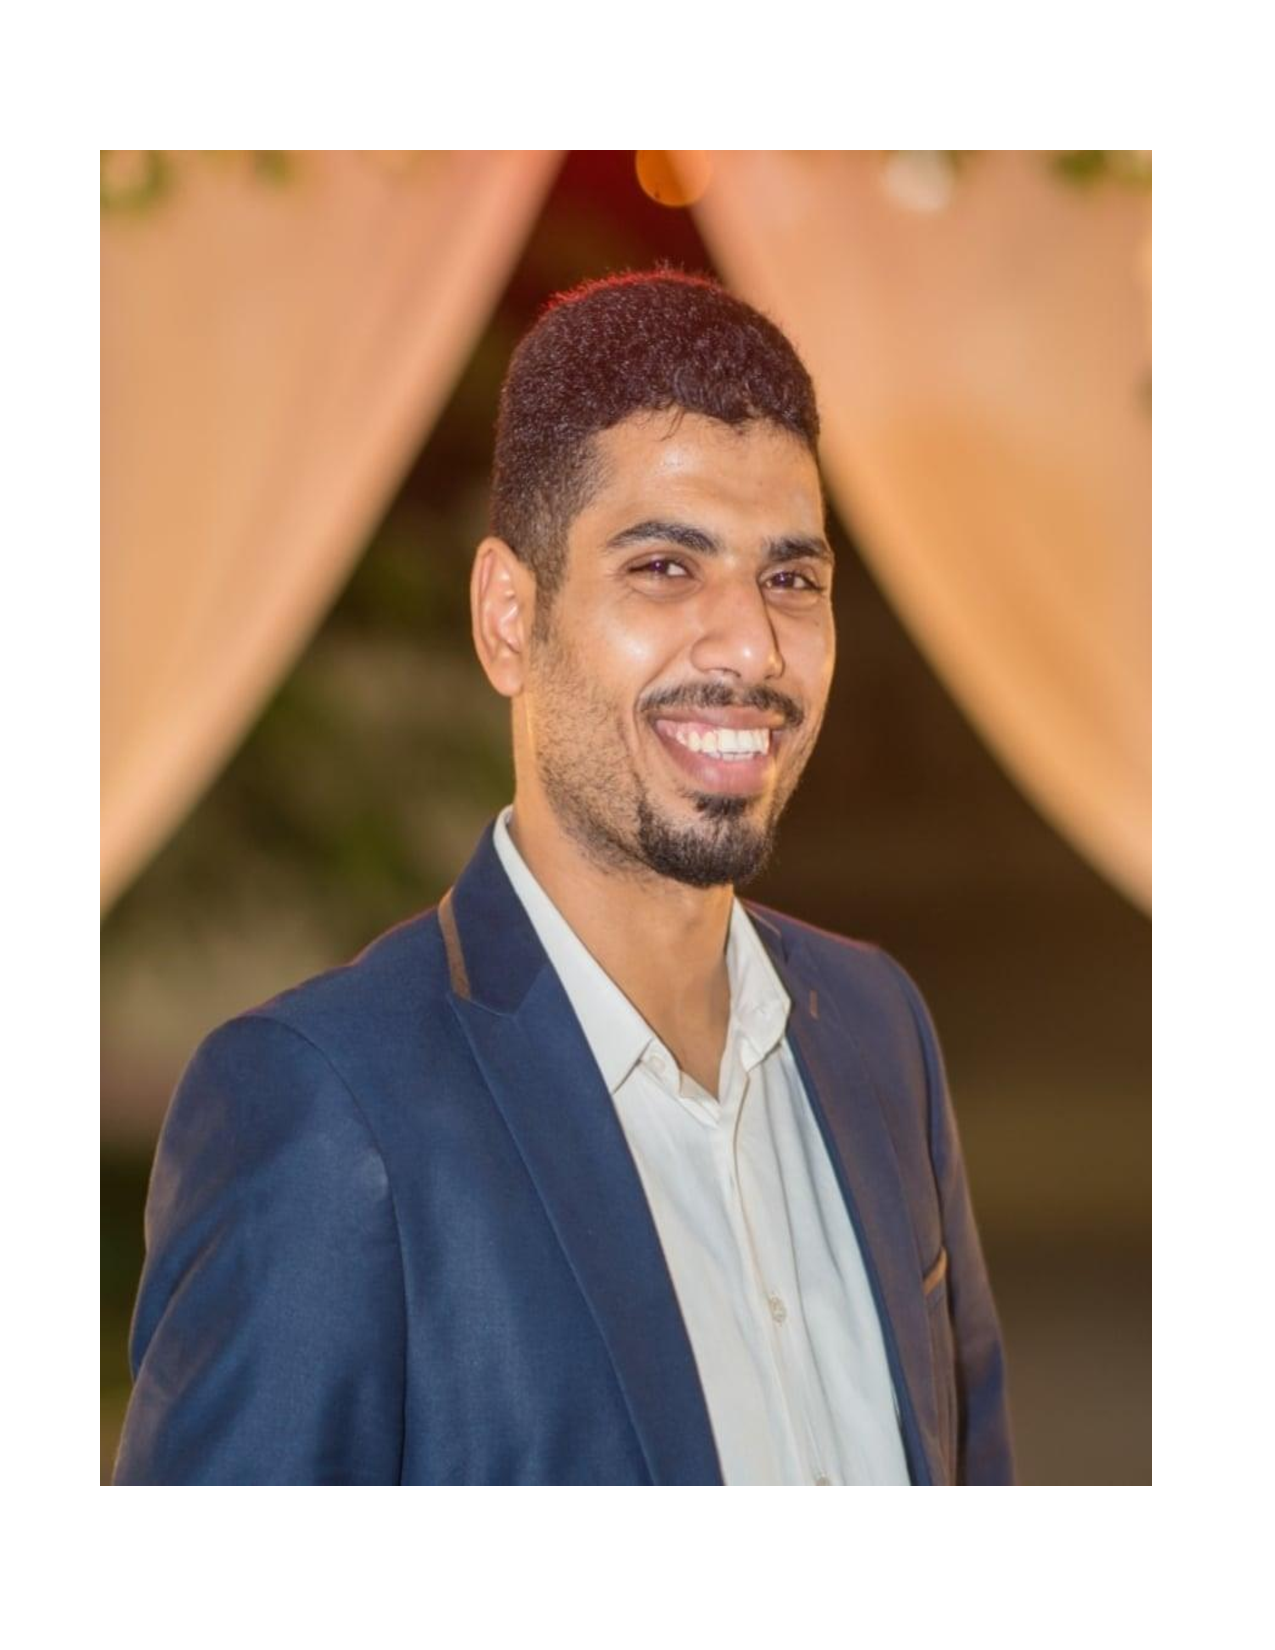
\includegraphics[width=0.6\columnwidth]{photo.pdf}
	\vspace{-7cm}
\end{figure}

\begin{flushright}\Small
	Shrief Abdelazeez \\
	\url{shrief.s.abdelazeez@eng1.cu.edu.eg}  \\
     Tel: +201158159448
\end{flushright}\normalsize
\framebreak


% Right frame
%%%%%%%%%%%%%%%%%%%%
\Huge\bfseries {\color{RoyalBlue} Shrief Abdelazeez} \\
\Large\bfseries  Biomedical Algorithm Software Engineer \\

\normalsize\normalfont

% About me
\begin{AboutMe}
Experienced Biomedical Algorithm Software Engineer eager to use my experience in this field to serve the community and industry. I got my Bachelor degree from Faculty of Engineering Cairo University, System and Biomedical Engineering Department. My cumulative grade was excellent with honor with GPA 3.9. Then, i have finished my pre-master subjects with excellent grade and GPA 4.0. Finally, i have gotten my master degree in the field of Artificial Intelligence (AI)in Healthcare from the Faculty of Engineering Cairo University. My research interests are Machine/Deep learning Algorithms, Natural Language Processing (NLP), Artificial Intelligence (AI) Algorithms, Statistical Analysis, Mathematical Modeling, Digital Signal Processing (DSP) Algorithms, Medical Imaging Technologies, Image Processing Algorithms, Image Registration Algorithms, Control Systems Algorithms, Adaptive Control Algorithms, Stochastic Processes Algorithms, and High Performance Computing (HPC).
\end{AboutMe}

% Experience
\CVSection{Work Experience}
\CVItem{July 2021 - present}\\
\begin{itemize}
  \item Assistant Lecturer at Faculty of Engineering Cairo University, System \& Biomedical Engineering Department.
  \item Senior \& Team Lead Algorithm Software Engineer at BioBusiness Company
\end{itemize}
\SmallSep
\CVItem{July 2020 - July 2021}\\
\begin{itemize}
  \item Teacher Assistant (TA) and Demonstrator at Faculty of Engineering Cairo University, System \& Biomedical Engineering Department.
  \item Junior Algorithm Software Engineer at BioBusiness Company
\end{itemize}
\SmallSep
\CVItem{Jan 2017 - Jun 2020}\\
\begin{itemize}
  \item Teacher Assistant (TA) and Demonstrator at Faculty of Engineering Cairo University,System \& Biomedical Engineering Department.
  \item Senior Test Engineer at Medical Equipment Calibration Lab (MECL).
\end{itemize}
\SmallSep

\CVItem{July 2016 - August 2016}\\
\begin{itemize}
  \item Service Engineer Trainee at Siemens Company.
  \item Maintenance and installation processes for MRI, CT Equipment.
\end{itemize}
\Sep


\clearpage
\framebreak
\framebreak
% Training & Courses
\CVSection{Training \& Courses}
\CVItem{Jan 2020 - Jun 2020}\\
Deep learning course from Udacity using Pytorch.\\

\CVItem{Jan 2015 - May 2015}\\
\CVItem{C++ Course at Smart Apps Company}
\begin{itemize}
  \item Object Oriented Programming Concepts.
  \item Templates and Standard Template Library (STL).
\end{itemize}

\CVItem{Aug 2014 - Oct 2014}\\
\CVItem{C Programming Language Under Linux at Smart Apps Company}\\
Working under linux operating environment using c programming language.\\
\Sep

\CVItem{July 2014 - Aug 2014}\\
\CVItem{Trainee at El Gomhoria Company}
\begin{itemize}
  \item Monitors.
  \item Spectrophotometer.
  \item X-ray.
\end{itemize}
\Sep




% Education
\CVSection{Education}
\CVItem{Master of Science in Systems \& Biomedical Engineering at \textbf{Faculty Of Engineering, Cairo University} 2017 - 2021}\\
\textit{Title}: "Transfer learning based framework for Multi class classifications of breast cancer using  Whole Slide Images (WSIs)".\newline
\SmallSep


\CVItem{Bachelor Degree - System \& Biomedical Engineering at \textbf{Faculty Of Engineering, Cairo University}, 2011 - 2016}\\
\begin{itemize}
  \item Excellent Degree with honor.
  \item \textbf{Graduation Project}:High Performance Distributed Volume Rendering on Heterogenous Platforms.
  \item Excellent Degree for Graduation Project.
  \item My rank is third of class.
  \item My GPA is 3.9.
\end{itemize}
\Sep



% Skills
\CVSection{Skills}
\CVItem{Programming Skills}
\begin{multicols}{3}
\begin{compactitem}[\color{RoyalBlue}$\circ$]
	\item C/C++ 
	\item Qt Creator
	\item Matlab
	\item MySQL
	\item OpenMP
	\item OpenCL
	\item Python
	\item Pytorch
	\item Latex
	\item Git 
	\item CMake
\end{compactitem}
\end{multicols}
\SmallSep

\clearpage
\framebreak
\framebreak

\CVSection{Projects}\\
\CVItem{Projects Associated to BioBusiness Company}
\begin{enumerate}
\item \textbf{Inspector V4 Device, 2022} 
\begin{itemize}
\item DSP algorithms for detection and monitoring of power quality event disturbances such as Transient, Rapid Voltage Change (RVC), Interruption, DIP, SWELL, and frequency.
\item Calculation and monitoring of power parameters such as active, reactive, and apparent power, True power factor, Displacement power factor, Crest factor, phase unbalance, Total harmonis distortions... etc
\end{itemize}

\item \textbf{Desktop application for system calibration of BioVent A-series device using .Net , 2022} 
\begin{itemize}
\item Design the front-end user interface for the desktop application
\item Develop the back-end algorithms using .Net framework
\item USB serial communication protocol for transmitting and receiving data between the device and PC
\end{itemize}
\item \textbf{Non-Invasive Ventilator (NIV) Modes, BioVent A-series device project , 2022}
\begin{itemize}
	\item Mathematical modeling for Pressure signal driven from the blower used in the device using Matlab (Simulink)
	\item Design PID controller to control pressure out from the blower using Matlab (Simulink) 
    \item Design Continuous Positive Airway Pressure (CPAP) mode algorithm 
    \item Design Auto-CPAP mode algorithms 
    \item Design Bi-Level-Spontaneous Positive Airway Pressure (BiPAP -S) mode algorithms 
    \item Design Bi-Level-Spontaneous and Time Positive Airway Pressure (BiPAP -ST) mode algorithms 
    \item Design Bi-Level Volume Target (BiPAP -VT) mode algorithms 
    \item Design Pressure Controlled Ventilation (PCV) mode algorithms 
    \item Design Pressure Support Ventilation (PSV) mode algorithms 
    \item Moving Average Low Pass Filter algorithm to get rid of noise associated to the pressure and flow sensors
\end{itemize}
\item \textbf{High Flow Nasal Canula (HFNC) Project, 2021}
\begin{itemize}
    \item Mathematical modeling for flow signal driven from the blower used in the device using Matlab (Simulink) 
    \item Design PID controller to control mix flow using Matlab \& C 
    \item Non-linear mathematical model for oxygen flow signal driven from the  proportional valve used in the device using Matlab (Simulink) 
    \item Design PID cascade controller to control flow driven from the proportional valve using Matlab \& C  
    \item Developing an algorithm in order to detect tube obstruction or disconnection 
\end{itemize}
\end{enumerate}



\clearpage
\framebreak
\framebreak
\CVItem{Projects Associated to Faculty of Engineering Cairo University, System \& Biomedical Engineering Department}
\begin{enumerate}

\item \textbf{Master Project, Transfer learning algorithm for multi-class classification of breast cancer whole slide microscopic images using PyTorch, 2019 - 2021}
\begin{itemize}
\item Image preprocessing using Torchvision Package.
\item Image augmentation techniques using ImageDataGenerator in Keras.
\item Use DenseNet201 as a pretrained model and adding my proposed classifier model
\item Using combination between Adam algorithm and step decay scheduler as an optimization technique.
\item Training the model on cloud computing using Colab.
\item Testing the model empirically and achieving average accuracy 95\%
\end{itemize}
\item \textbf{Graduation Project, High Performance Distributed Volume Rendering on Heterogeneous Computing Platforms, 2016}
\begin{itemize}
\item An efficient rendering pipeline targeting interactive volume rendering of large scale volumes that are acquired by advanced state-of-the-art medical scanners, and cannot fit on the memory of single rendering device.
\item  Multi-GPU framework that is suitable for clinics equipped by Multi-GPU workstations, and for mid-size volumes.
\item Cluster implementation for large radiology stations to handle very large scale volumes.
\item Implemented both sort-first and sort-last parallel rendering techniques to handle different types of processing for different applications.
\end{itemize}
\item \textbf{Computer Vision Project, Face Recognition using Principle Component Analysis (PCA) and Sum of Square Difference (SSD), 2016}
\begin{itemize}
\item Image preprocessing.
\item  Extract eigenfaces features using PCA.
\item Use SSD as a classifier.
\item Plotting ROC curve to evaluate the performance of the model.
\end{itemize}
\item \textbf{Bio-statistics Project, ECG binary classification using energy feature extraction and KNN classifier, 2014}
\begin{itemize}
\item Signal preprocessing such as low pass filter to remove the noise.
\item  Extract features using energy of the signals.
\item Classify the ECG signal into normal or abnormal using KNN classifier.
\item Evaluate the model based on some metrics such as accuracy, sensitivity, and Specificity.
\end{itemize}
\end{enumerate}


\Sep

\clearpage
\framebreak
\framebreak


\CVSection{Publications}
\begin{enumerate}
\item \CVItem{Paper in EMBC 2016}:\textit{ "Parallel generation of digitally reconstructed radiographs on heterogeneous multi-GPU workstations," 38th Annual International Conference of the IEEE Engineering in Medicine and Biology Society (EMBC), 2016.}
\item \CVItem{Paper in ISC 2015}:\textit{"Speaker Recognition Using MFCC and Vector Quatization," Annual International Student Conference of Biomedical Engineering (ISC), 2015}, 2nd best paper.
\end{enumerate}
\Sep

\CVSection{Awards}
\CVItem{2nd best Paper in the International Student Conference (ISC), 2015}
\textbf{Title}:\textit{"Speaker Recognition Using MFCC and Vector Quatization"}\newline
\Sep

\CVSection{Certificates}
\begin{itemize}
\item \CVItem{Master Degree}: Master Of Science in Biomedical Engineering \& Systems, 2022 (\href{https://drive.google.com/file/d/1giRjSlg57sNPhUK0scea5JC0JahuYhVl/view?usp=sharing}{Link})
\item \CVItem{Sololearn}: HTML Course, 2021 (\href{https://www.sololearn.com/Certificate/1014-20775781/jpg/}{Link})
\item \CVItem{Test Automation University}: Java Programming Course, 2021 (\href{https://firebasestorage.googleapis.com/v0/b/testautomationu-9e0b6.appspot.com/o/certificates%2FTAU-38eb3fba.png?alt=media&token=d50fb732-d2bd-451f-9c6c-a5679299aca0}{Link})
\item \CVItem{Bachelor Degree}: Biomedical \& System Engineering, 2016 (\href{https://drive.google.com/file/d/1gmelA3pLTxUbTTkS7VY0o8f30b0lenkS/view?usp=sharing}{Link})
\end{itemize}
\\
% References
\CVSection{Language Skills}
\begin{enumerate}
\item \CVItem{Arabic}: Native Language.
\item \CVItem{English}: Excellent.
\item \CVItem{Deutsch}: A1.1.
\end{enumerate}
\Sep


% References
\CVSection{References}
References upon request.

%%%%%%%%%%%%%%%%%%%%%%%%%%%%%%%%%%%%%
% End document
%%%%%%%%%%%%%%%%%%%%%%%%%%%%%%%%%%%%%
\end{document}